\documentclass[10pt]{article}
\usepackage{icmlko}

\icmlmeta{IP 파운데이션 월드모델}{11}{축은 변해야 쓸모가 있다}{시간 추세를 빼도 전이는 살아남는다 --- 그리고 왜 옛날에는 통하지 않았는지가 드러난다}

\begin{document}

\twocolumn[
\icmlheader

\begin{abstract}
노트 10은 굿즈 규모가 팝업에서 아이돌로 유의하게 전이된다고 보고했다(차이 $-$0.0556,
순열 p=0.034). 그 뒤 데뷔 연도 구간별로 쪼개 보니 최근 구간에서만 이겼다 ---
2021년 이전 $+$0.1451, 2022--2024 $+$0.0565, 2025년 이후 $-$0.0226. 시간 혼동을
의심할 만한 신호였고, 실제로 공통 추세가 있었다(연도와 굿즈 규모 r=$+$0.386,
연도와 초동 r=$+$0.426). 양쪽 도메인에서 선형 시간 추세를 빼고 다시 쟀다.
\textbf{전이는 살아남는다} --- 차이 $-$0.0435, 순열 p=0.0343, 계수 $+$0.213에서
$+$0.216으로 사실상 불변이다. 효과 크기만 22\% 줄어들므로 노트 10의 수치를
정정한다. 더 흥미로운 것은 구간별 결과다. 추세를 빼자 초기 구간의 큰 손실이
거의 사라진다($+$0.1451 $\to$ $+$0.0148). 손해가 아니라 \emph{무효}였던 것이다.
이유는 축의 분산에 있다. 2019--2021년 데뷔 앨범은 평균 1.88종이고 축 표준편차가
0.154였다 --- 거의 모두가 1--2종이라 축이 변하지 않았다. 2025년 이후는 평균 3.29종,
표준편차 0.231이다. \textbf{축은 그 모집단에서 변해야 예측할 수 있다.} 도메인
불변성과는 별개의 조건이며, 파운데이션 모델이 어느 시기·어느 도메인에 적용
가능한지를 가르는 기준이 된다. 부수적으로 타깃 폭 축의 결측 처리 버그를 발견해
고쳤다.
\end{abstract}
]

\section{의심스러운 신호}

노트 10은 첫 도메인 간 전이를 보고했다. 그 직후 시간 안정성을 점검했다 --- 효과가
전 기간에 고르게 있는지, 아니면 특정 시기에만 있는지.

\begin{table}[t]
\centering\tsize
\caption{굿즈 규모 팝업 $\to$ 아이돌, 데뷔 연도 구간별 (추세 제거 전).}
\begin{tabular}{lrr}
\toprule
구간 & n & 차이 \\
\midrule
2021년 이전 & 20 & $+$0.1451 \\
2022--2024 & 23 & $+$0.0565 \\
2025년 이후 & 26 & $-$0.0226 \\
\bottomrule
\end{tabular}
\end{table}

통합하면 $-$0.0556으로 이기는데 세 구간 중 둘이 진다. 통합 성적이 구간 내 성적보다
좋다면 효과가 \emph{구간 사이}에 있다는 뜻이고, 그것은 축의 관계가 아니라 시간
추세일 수 있다.

확인했다. 공통 추세가 실재했다.

\begin{table}[t]
\centering\tsize
\caption{아이돌 풀(n=67)의 상관 구조.}
\begin{tabular}{lr}
\toprule
쌍 & r \\
\midrule
연도 $\times$ 굿즈 규모 & $+$0.386 \\
연도 $\times$ 초동 & $+$0.426 \\
굿즈 규모 $\times$ 초동 & $+$0.432 \\
\midrule
\textbf{연도 통제 후 부분상관} & \textbf{$+$0.321} \\
\bottomrule
\end{tabular}
\end{table}

앨범 버전 수도 초동도 함께 늘어왔다. 다만 관계가 통째로 추세는 아니다 --- 연도를
통제한 부분상관이 $+$0.321로 원래 $+$0.432의 74\%가 남는다.

\section{추세를 빼고 다시 쟀다}

양쪽 도메인에서 각각 선형 시간 추세를 뺐다. 한쪽만 빼면 눈금이 어긋나므로 팝업
쪽도 데뷔 연도로 같은 처리를 했다.

\begin{table}[t]
\centering\tsize
\caption{굿즈 규모 단독, 팝업 $\to$ 아이돌. 순열 4,000회, 부트스트랩 2,000회.}
\begin{tabular}{lrr}
\toprule
& 원본 & 추세 제거 \\
\midrule
차이 & $-$0.0556 & $-$0.0435 \\
순열 p & 0.0340 & 0.0343 \\
부트 이긴 비율 & 94\% & 94\% \\
팝업 계수 & $+$0.213 & $+$0.216 \\
\bottomrule
\end{tabular}
\end{table}

\begin{figure}[t]
\centering
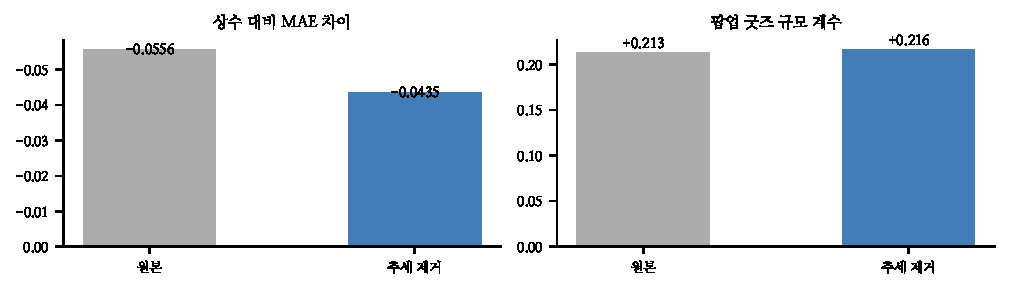
\includegraphics[width=\textwidth]{figs/effect.pdf}
\caption{효과 크기는 22\% 줄지만 계수는 그대로다. 추세가 실어 준 것은 크기이지
관계 자체가 아니다.}
\end{figure}

전이는 살아남는다. 순열 p가 0.0340에서 0.0343으로 거의 움직이지 않고, 팝업에서
추정한 계수는 $+$0.213에서 $+$0.216으로 사실상 같다. 시간 추세가 실어 준 것은
\emph{효과의 크기}이지 관계 자체가 아니었다.

\claimx{노트 10의 전이는 시간 인공물이 아니다. 양쪽 도메인에서 선형 추세를 제거한
뒤에도 순열 p=0.0343으로 유의하며 계수가 불변이다. 다만 효과 크기는
$-$0.0556에서 $-$0.0435로 정정한다.}{2차 이상의 시간 항이나 시장 규모 같은
공변량을 추가로 통제했을 때 p가 0.05를 넘으면 선형 탈추세가 부족했던 것이다.}

\section{그런데 구간별 결과가 더 흥미롭다}

같은 탈추세를 구간별 검정에 적용했다.

\begin{table}[t]
\centering\tsize
\caption{구간별, 추세 제거 전후.}
\begin{tabular}{lrrr}
\toprule
구간 & n & 원본 & 추세 제거 \\
\midrule
2021년 이전 & 20 & $+$0.1451 & $+$0.0148 \\
2022--2024 & 23 & $+$0.0565 & $+$0.0295 \\
2025년 이후 & 26 & $-$0.0226 & $-$0.0759 \\
\bottomrule
\end{tabular}
\end{table}

\begin{figure}[t]
\centering
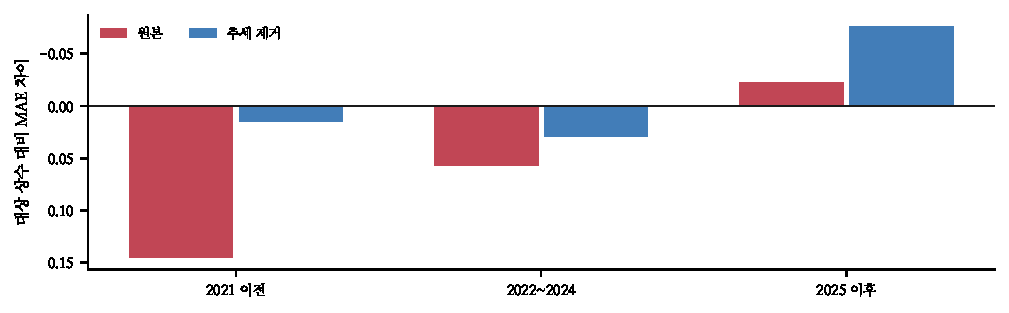
\includegraphics[width=\textwidth]{figs/detrend.pdf}
\caption{추세를 빼자 초기 구간의 큰 손실이 거의 사라지고 최근 구간은 오히려
강해진다. 초기 구간은 손해가 아니라 무효였다.}
\end{figure}

초기 구간의 $+$0.1451이 $+$0.0148로 줄었다. 거의 0이다. 즉 그 시기에 축이
\emph{틀린} 것이 아니라 \emph{아무것도 말하지 않은} 것이다. 반대로 최근 구간은
$-$0.0226에서 $-$0.0759로 세 배 이상 강해졌다.

\section{왜 옛날에는 통하지 않았나}

축의 분산을 봤다.

\begin{table}[t]
\centering\tsize
\caption{구간별 굿즈 규모 축의 분포와 앨범 버전 수.}
\begin{tabular}{lrrrr}
\toprule
구간 & n & 축 평균 & 축 표준편차 & 버전 평균 \\
\midrule
2021년 이전 & 16 & 0.253 & 0.154 & 1.88 \\
2022--2024 & 23 & 0.329 & 0.196 & 2.61 \\
2025년 이후 & 24 & 0.482 & 0.231 & 3.29 \\
\bottomrule
\end{tabular}
\end{table}

\begin{figure}[t]
\centering
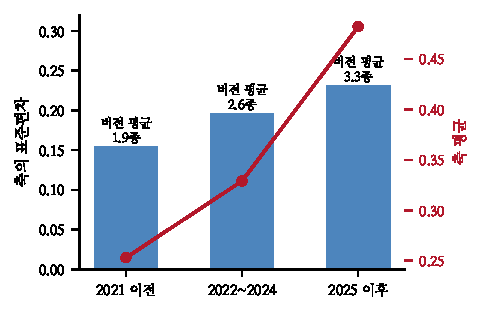
\includegraphics[width=\columnwidth]{figs/variance.pdf}
\caption{축의 표준편차가 0.154에서 0.231로 50\% 늘었다. 선은 축의 평균이다.
버전 수 경쟁이 축에 변별력을 준 셈이다.}
\end{figure}

2019--2021년 데뷔 앨범은 평균 1.88종이었다. 거의 모두가 1종이나 2종이었으므로
``굿즈 규모''라는 축은 사실상 상수였다. 상수는 아무것도 예측하지 못한다. 그
이후 버전 경쟁이 벌어지면서 평균이 3.29종까지 올랐고 축의 표준편차가 50\% 늘었다.

이것은 계수가 틀렸다는 뜻이 아니다. 팝업에서 배운 계수 $+$0.216은 두 시기에
똑같이 적용됐는데, 곱해질 입력이 변하지 않으면 예측도 변하지 않는다.

\claimx{축의 예측력은 그 축이 대상 모집단에서 얼마나 변하는가에 달려 있다.
도메인 불변성과는 별개의 조건이다 --- 계수가 옳아도 축이 상수면 쓸모가 없다.}{다른
축에서도 같은 패턴이 보여야 한다. 축의 구간 내 표준편차와 그 구간의 전이 성적이
상관되지 않으면 이 설명은 이 축 하나에만 해당하는 우연이다.}

\subsection{파운데이션 모델에 대한 함의}

이 조건은 실무적으로 중요하다. 공유 축을 확정했다 해도 그것을 아무 데나 적용할
수 없다는 뜻이기 때문이다. 새 도메인이나 새 시기에 모델을 붙이기 전에 물어야 할
것이 하나 늘었다.

\begin{quote}\fontsize{9.2}{11}\selectfont
\textbf{첫째,} 이 도메인에서 축이 같은 부호로 작동하는가 (노트 9--10).\\[0.3em]
\textbf{둘째,} 축 측정의 신뢰도가 문턱을 넘는가 (노트 9, r$\geq$0.79).\\[0.3em]
\textbf{셋째,} 이 모집단에서 축이 충분히 변하는가 (이 노트).
\end{quote}

셋째 조건은 사전에 라벨 없이 확인할 수 있다는 장점이 있다. 축 값만 재보면 되기
때문이다. 적용 가능성 점검의 첫 관문으로 쓸 수 있다.

\section{부수 발견 --- 타깃 폭의 결측 처리 버그}

타깃 폭 축을 다시 짜다가 오류를 찾았다. 아이돌 레코드의 \texttt{survival\_show}
필드는 값이 ``프로그램 이름 또는 None''인데, None을 \emph{결측}으로 처리하고
있었다. 그러면 관측된 44건이 전부 1.0이 되어 분산이 0이 된다. None은 결측이
아니라 ``서바이벌 출신 아님''이다.

성분별로 초동과의 상관을 재보니 기존 합성의 문제가 더 드러났다.

\begin{table}[t]
\centering\tsize
\caption{타깃 폭 성분별 초동과의 상관. 팝업 계수는 $+$0.336(양수)이다.}
\begin{tabular}{lrr}
\toprule
성분 & n & r \\
\midrule
사전 화제 기록 & 81 & $+$0.258 \\
인원 수 & 71 & $+$0.010 \\
혼성 여부 & 74 & $-$0.038 \\
걸그룹 여부 & 74 & $-$0.283 \\
\midrule
기존 합성 & 74 & $+$0.043 \\
\textbf{새 합성} & 81 & \textbf{$+$0.137} \\
\hspace{1em}연도 통제 후 & & \textbf{$+$0.180} \\
\bottomrule
\end{tabular}
\end{table}

기존 합성은 인원 수가 지배했는데 인원 수와 초동의 상관이 $+$0.010으로 사실상
0이다. 서바이벌 출신과 사전 화제 기록 --- 둘 다 ``데뷔 전에 얼마나 많은 사람에게
닿았는가''를 잰다 --- 으로 다시 만들자 $+$0.137, 연도 통제 후 $+$0.180이 됐다.
개선됐지만 여전히 약하다.

\paragraph{걸그룹 여부는 넣지 않았다}
상관이 $-$0.283으로 가장 강하지만 그것은 ``타깃 폭''이 아니라 시장 구조다 ---
보이그룹 팬덤의 음반 구매량이 크다는 것은 잘 알려져 있다. 축 이름과 다른 것을
넣으면 예측은 좋아져도 전이 해석이 망가진다. 축은 예측 성능이 아니라 의미로
정의된다.

\section{한계}

\begin{itemize}[leftmargin=1.1em,itemsep=0.15em]
\item 탈추세는 선형만 했다. 시장 규모나 코로나 같은 구조 변화는 선형이 아니다.
\item 구간별 n이 16--26이다. 구간 내 검정은 검정력이 낮다.
\item 축 분산과 예측력의 관계는 축 하나에서 본 것이다. 다른 축에서도 같은
      패턴이 나와야 일반 원리로 말할 수 있다.
\item 새 타깃 폭도 여전히 약하다($+$0.180). 전이 검정에 넣을 수준은 아니다.
\end{itemize}

\section{다음}

\begin{enumerate}[leftmargin=1.3em,itemsep=0.15em]
\item 축 분산과 전이 성적의 관계를 다른 축·다른 분할에서 재확인.
\item 새 타깃 폭으로 아이돌 축 갱신 후 전이 재검정.
\item 아이돌 굿즈 규모를 사람 태깅으로 다시 매기고 신뢰도 측정 --- 노트 10의
      비대칭 설명 검정.
\item 세 번째 도메인 확보. 두 도메인으로는 불변을 말하기 이르다.
\end{enumerate}

\vspace{0.6em}
\hrule height 0.3pt
\vspace{0.5em}
{\footnotesize
\textbf{참고문헌}\\[0.3em]
Good, P. (2005). \emph{Permutation, Parametric, and Bootstrap Tests of Hypotheses},
3rd ed. Springer.\\[0.15em]
Hernán, M. A., Robins, J. M. (2020). \emph{Causal Inference: What If}.
Chapman \& Hall.\\[0.15em]
Simpson, E. H. (1951). The interpretation of interaction in contingency tables.
\emph{JRSS B}, 13(2), 238--241.\\[0.15em]
Ben-David, S. et al. (2010). A theory of learning from different domains.
\emph{Machine Learning}, 79(1--2), 151--175.
}

\end{document}
